\section{実験装置}
\subsection{液体酸素(LOX)}
液体酸素(LOX)の基本的な物性値をTable2-1に、液体酸素の飽和蒸気圧と潜熱、密度を温度の関数としてそれぞれFig.2-およびFig.2-に示す。
\begin{figure}
\centering
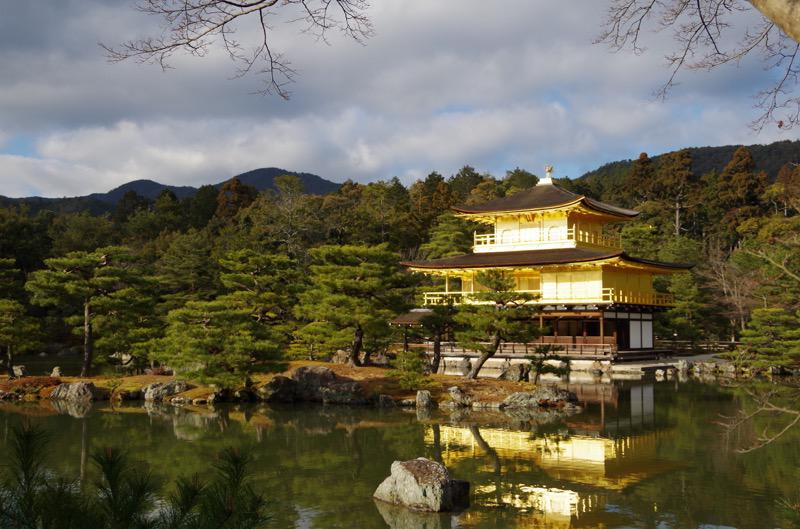
\includegraphics[width=5cm]{apple.png}
\caption{TestPic}
\end{figure}
\subsection{アクリル樹脂(PMMA)}
本実験で用いる燃料はアクリル樹脂(PMMA)とした。アクリル樹脂の基本的な物性値をTable2-2に示す。

\subsection{プリバーナ方式液体酸素気化器}
本実験では2種類の気化器を使用した。
気化器1は気化器内部の状態を可視化するために、アクリル樹脂と石英ガラスを使用した。

気化器2は基礎データ取得のために、ステンレスとグラファイトを使用した。
各気化器の外観をFig.2-に示す。

%\subsection{アクリル樹脂(PMMA)}
本実験で用いる燃料はアクリル樹脂(PMMA)とした。アクリル樹脂の基本的な物性値をTable2-2に示す。


